% ============================================================
% replica of the original Word document
%  Font: Times New Roman | Page: A4 | Layout: 2-column
%  Original: 5 pages
% ============================================================
\documentclass[10pt,a4paper]{article}

\usepackage[T1]{fontenc}
\usepackage[utf8]{inputenc}
\usepackage{mathptmx}          % Times New Roman
\usepackage{microtype}

% Page geometry matching original Word doc exactly
% w=11906 twips, h=16838 twips (A4)
% top=540, bottom=1440, left=893, right=893 twips
% 1 inch = 1440 twips = 2.54 cm
\usepackage[
  a4paper,
  top=0.953cm,
  bottom=2.54cm,
  left=1.576cm,
  right=1.576cm,
  columnsep=1.27cm,
  headsep=0pt,
  headheight=0pt,
  footskip=1.0cm
]{geometry}

\usepackage{multicol}
\usepackage{graphicx}
\usepackage{array}
\usepackage{tabularx}
\usepackage{booktabs}
\usepackage{caption}
\usepackage{enumitem}
\usepackage{titlesec}
\usepackage{fancyhdr}
\usepackage{setspace}
\usepackage[hidelinks]{hyperref}
\usepackage{tikz}
\usetikzlibrary{shapes.geometric, arrows.meta, positioning, calc}

% ── Body font: 10pt / 12pt leading (Word default) ──────────
\renewcommand{\normalsize}{\fontsize{10}{12}\selectfont}
\normalsize

% ── Paragraph spacing: 6pt after each paragraph (120 twips / 20 = 6pt) ──
\setlength{\parindent}{0.48cm}
\setlength{\parskip}{6pt}

% ── Section headings ─────────────────────────────────────────
\titleformat{\section}[block]
  {\normalfont\fontsize{10}{12}\selectfont\scshape\centering}
  {\Roman{section}.}{0.4em}{\MakeUppercase}
\titlespacing*{\section}{0pt}{6pt}{2pt}

% Subsections: "A.  Title" italic
\titleformat{\subsection}[block]
  {\normalfont\fontsize{10}{12}\selectfont\itshape}
  {\Alph{subsection}.}{0.5em}{}
\titlespacing*{\subsection}{0pt}{4pt}{1pt}

% ── Lists ────────────────────────────────────────────────────
\setlist[enumerate,1]{
  leftmargin=1.5em, label=\arabic*.,
  topsep=2pt, itemsep=1pt, parsep=0pt, partopsep=0pt
}
\setlist[itemize,1]{
  leftmargin=1.5em,
  topsep=2pt, itemsep=1pt, parsep=0pt, partopsep=0pt,
  label=\textbullet
}
\setlist[enumerate,2]{
  leftmargin=2.2em, label=\alph*.,
  topsep=1pt, itemsep=0pt, parsep=0pt
}

% ── Captions ─────────────────────────────────────────────────
\captionsetup{
  labelformat=empty,
  font={normalsize},
  justification=centering,
  skip=2pt
}
\usepackage{graphicx}
% ── Footer ───────────────────────────────────────────────────
\pagestyle{fancy}
\fancyhf{}
\fancyfoot[L]{\fontsize{8}{10}\selectfont }
\renewcommand{\headrulewidth}{0pt}
\renewcommand{\footrulewidth}{0pt}

% ════════════════════════════════════════════════════════════
\begin{document}
% ════════════════════════════════════════════════════════════

% ─────────────────────────────────────────────────────────────
%  TITLE  (full width, single column before multicols)
% ─────────────────────────────────────────────────────────────
{\centering
\fontsize{22}{27}\selectfont\setlength{\parskip}{0pt}
A Machine Learning Framework for Stress Detection During Social Media Usage Using Wearable Physiological Signals\par
}

\vspace{6pt}
\setlength{\parskip}{0pt}

% Author table
{\centering\fontsize{9}{11}\selectfont
\begin{tabular}{p{5.5cm}p{5.5cm}p{5.5cm}}
  \centering Dr.\ Raghav Mehra
    & \centering Krish Latawa
    & \centering\arraybackslash Omika Gupta \\[1pt]
  \centering raghav.mehrain@gmail.com
    & \centering krishlatawa05@gmail.com
    & \centering\arraybackslash omika1321gupta@gmail.com \\[1pt]
  \centering AIT-CSE, Chandigarh University, Mohali, Punjab
    & \centering AIT-CSE, Chandigarh University, Mohali, Punjab
    & \centering\arraybackslash AIT-CSE, Chandigarh University, Mohali, Punjab \\[6pt]
    \\
  \centering Harmanpreet Kaur
    & \centering Kaushik
    & \\[1pt]
  \centering iharmansaini51@gmail.com
    & \centering kaushik95873@gmail.com
    & \\[1pt]
  \centering AIT-CSE, Chandigarh University, Mohali, Punjab
    & \centering AIT-CSE, Chandigarh University, Mohali, Punjab
    & \\
\end{tabular}\par
}

\vspace{8pt}
\setlength{\parskip}{6pt}

% ─────────────────────────────────────────────────────────────
%  TWO-COLUMN BODY
% ─────────────────────────────────────────────────────────────
\begin{multicols}{2}

% ── Abstract ─────────────────────────────────────────────────
\fontsize{10}{12}\selectfont
\noindent\textbf{Abstract\textemdash} Stress has a substantial impact on both physical and mental health, but current detection techniques only use social media posts or physiological signals, both of which come with significant drawbacks. This study suggests a machine learning-based framework that integrates real-time physiological data from wearable devices with social media usage patterns. The system focuses on identifying early behavioural and physiological indicators of stress before severe symptoms appear. The proposed framework facilitates early stress detection and supports real-time stress monitoring. Experimental results demonstrate that the stacking ensemble achieved an accuracy of 89.6\%, with an F1-score of 88.1\%, outperforming individual classifiers by 2\textendash7\%.

\noindent\textit{Keywords\textemdash} Stress detection, machine learning, wearable devices, physiological signals, social media analysis, and mental health monitoring.

% ── I. INTRODUCTION ──────────────────────────────────────────
\section{Introduction}

\fontsize{10}{12}\selectfont

Stress refers to a physiological and psychological response that occurs when individuals perceive an imbalance between environmental demands and coping capacity. Excessive stress can primarily lead to numerous negative consequences, including anxiety, depression, heart diseases such as high blood pressure, heart attack, stroke, as well as weakened immunity, and hormonal imbalances. The autonomic nervous system  controls your heart rate, breathing, vision changes and more. Its built-in stress response commonly known as the fight or flight response, helps the body to adapt to stressful situations.

Several physiological markers have been extensively studied for stress detection. Heart Rate Variability (HRV), which represents the variation in time intervals between consecutive heartbeats, serves as a key indicator of autonomic balance. Reduced HRV is commonly associated with sympathetic dominance and heightened stress, whereas elevated HRV reflects parasympathetic regulation and improved stress resilience. Electroencephalogram (EEG) signals also provide insights into neural activity patterns, as stress-related conditions are associated with alterations in specific frequency bands. Additionally, electrodermal activity (EDA) and other bio signals have demonstrated strong correlations with emotional arousal and stress responses.


The objective of this paper is to explore the application of ML methods in stress detection using the content people consume online and highlight the potential advantages and challenges associated with this approach. Most existing models detect stress using posts or comments made by users, but not the content they actually consume online on different platforms like articles, videos, reels on Instagram, news feed, articles or posts on X (Twitter).  This paper proposes the use of different machine learning models to predict stress based on the social media consumption patterns.

There are several challenges in detecting stress, and the number one challenge is that stress is subjective; two individuals may experience similar stress levels while exhibiting different physiological responses, and one of the signals that is consuming negative content online may also vary among different people. Furthermore, coping mechanisms differ, as some individuals engage in prolonged scrolling while other consume different forms of media.

Nowadays, people tend to show sign of stress online before admitting it themselves. People tend to increase their screen-time in order to distract themselves from the stress. Consequently, social media activity can provide early indicators of deteriorating mental health.

% ── II. CONTRIBUTIONS ────────────────────────────────────────
\section{Contributions}

The main contributions of this work are summarised as follows:

\begin{enumerate}
  \item A hybrid stress detection framework combining real-time physiological signals and passive social media content consumption.
  \item A personalised baseline mechanism to account for inter-user physiological variability.
  \item An ensemble and stacking-based machine learning approach that improves stress classification accuracy over individual models.
  \item An experimental evaluation on wearable sensor data collected under controlled conditions demonstrating improved robustness across stress levels.
\end{enumerate}

\noindent These contributions collectively enable early, non-intrusive stress detection by combining behavioral exposure and physiological responses.

% ── III. RELATED WORK AND NOVELTY ────────────────────────────
\section{Related Work and Novelty}

Before ML is incorporated, Researchers primarily examined physiological signals to predict the stress levels of the person. These biological signals include: - Heart Rate Variability (HRV), skin conductance (GSR), EEG and cortisol levels, etc. Also, in the field of ML \cite{ref1}
 Logistic regression was used on biological and contextual data, but due to its linearity, it didn't apply to complex stress patterns. SVM model \cite{ref2} used to detect stress from heart rate and skin conductance used handcrafted features (features designed by researcher from raw data). SVM model is not as scalable as other ML models. k-NN(k-Nearest Neighbours) is another model used by Hong Lu(Intel Lab), which used sensor- based data to predict the stress level of person. However, the model was sensitive to noise and couldn't work efficiently for large dataset. However, Decision Trees \cite{ref4} is one of the most convenient model in ML which is used to for emotion and stress classification and comes with the limitation of weak generalisation problem while training and testing of the dataset. Another model which is incorporated in one of the research done by Amir Muaremi and Bert Arnich \cite{ref5} used Random Forest as their ML model to predict stress levels from daily routine. However, their model comes with the limitation of using feature engineering to develop various features, including late-night screen-time ratio and doomscrolling score, etc.

Another model uses gradient boosting whose research is done by Y. Wang alongside his colleagues including A.T. Campbell and others. These scholars worked on these models based on constraints such as app usage and activity logs. However, their work is appreciable and predicted stress levels precisely but their model demonstrated limited generalization, indicating potential overfitting to the training data. Also, because of the complexity of the decision trees, the model was unable to predict the main reason behind the stress of the person. A.Saha and R.Sindhu \cite{ref7} also conducted research towards ``Sentiment analysis on Twitter data for stress detection'' which is a text-based model that predicts stress based on text-content of the twitter post of person. However, it also contains some limitations including future independence where the input features are treated as independent features and aren't related with each other. Also, this model has weak performance when complex human emotions are taken as input features.

Unlike existing studies that primarily rely on user-generated text or surveys, this study focuses on passive social media content consumption and synchronised physiological responses. The integration of personalised physiological baselines and ensemble learning enables robust stress detection. As a result, the proposed framework is more suitable for real-world and continuous stress monitoring scenarios.
Apart from traditional physiological signal based methods, many researchers have also worked on stress detection using mobile sensing and behaviour monitoring. Wang et al. \cite{ref6} developed a smartphone-based system in which stress level was predicted using mobile usage information such as activity logs, application usage, and contextual data collected from the device. Their results showed that behavioural data can help in understanding the mental condition of a person, but the accuracy of prediction depends on proper and continuous data collection.

In recent years, social media platforms have also been used for analysing mental health conditions. De Choudhury et al. \cite{ref8} analysed user behaviour on social networking sites and showed that posting patterns, interaction level, and online activity can be useful indicators of stress and depression. However, such techniques mainly depend on the text written by the user and do not consider the physical or physiological condition of the person.

More advanced approaches using deep learning have also been proposed to improve prediction performance. Ghosh and Anwar \cite{ref9} introduced a deep learning based model to estimate depression level from social media data. Their study showed that deep learning models are capable of identifying complex emotional patterns, but these methods require large datasets and higher computational power, which may not always be available.

Research based on wearable devices has also shown promising results in stress recognition. Sano and Picard \cite{ref10} used wearable sensors to record physiological signals such as heart rate, skin conductance, and body temperature for real-time stress detection. Their work proved that physiological signals provide more reliable information compared to questionnaires, but continuous monitoring through wearable devices is required.

A detailed review by Chancellor and De Choudhury \cite{ref11} explained different machine learning and deep learning techniques used for mental health prediction from online data. Their study suggested that better results can be achieved when multiple types of data are combined together instead of using only one source. However, most of the existing research either focuses only on physiological signals or only on social media activity.

Therefore, there is a strong need for a combined approach that can use both physiological signals and social media consumption behaviour for stress detection. Such a hybrid system can provide earlier and more accurate identification of stress conditions. The proposed work tries to fill this gap by combining wearable sensor data, social media exposure information, and ensemble-based machine learning techniques to improve the performance of stress classification.
% ── IV. METHODOLOGY ──────────────────────────────────────────
\section{Methodology}

Stress is a physiological and psychological response that arises from imbalance between individual responses and environmental demands. While acute stress may enhance the alertness and performance of an individual, chronic stress leads to mental degradation and system dysregulation.

The modern digital world has significantly changed the way people interact with the content available online. Continuous exposure to specific type of materials, such as academic stress, comparison-driven interviews and extended screen usage during late hours, can contribute to elevated stress levels. Stress detection started in the early to mid-2010s using wearable devices which detected the physiological signals like heartbeat and blood pressure. With the advancement in Machine Learning Algorithms in 2012 (Voice-Based Detection), smartphone and ambient sensors helped. Now with the emerging LLMs in 2023 the accuracy and recall of the models increased through advanced pattern recognition and contextual understanding.

Most of the stress detection studies focused on only the physiological signals using wearables and the text written by user. Limited attention is given to the type of content consumed and the behavioral consumption patterns, which represent passive yet influential factor of mental well-being.

Online platforms influence the mental well-being of the user due to the volume, frequency, and nature of content they deliver to the user. Individuals exposed to negative content have high chances of being marked as ` stressed.  Consequently, analysis of content consumption behavior presents a promising, less intrusive and scalable approach for stress detection. Content exposure was represented using predefined stimulus categories and exposure duration, and physiological responses were analyzed relative to exposure duration rather than semantic content analysis.

\subsection{System Overview}

The proposed methodology follows a multi model and ensemble-based approach to detect stress triggered by social media content consumed by user. The model has labels that represent physiological stress response,

not clinical validation. This model integrates physiological data from wearable sensors with machine learning models to detect stress in real-time. The overall workflow consists of five major stages:

\begin{enumerate}
  \item Physiological data collection using wearable sensors
  \item Signal preprocessing and noise removal
  \item Feature extraction and normalisation technique
  \item Ensemble learning based stress classification
  \item Model evaluation and performance
\end{enumerate}

\subsection{Physiological Data Acquisition}

Physiological signals are recorded while participants are exposed to social media content. The data is synchronized with content exposure timestamps to ensure accurate stress labeling.

Physiological data is collected using a sensor-based wearable device designed to be worn on the wrist. The Device contains multiple sensors to capture different stress-related attributes and respond accordingly.

{\setlength{\parskip}{0pt}
\begin{center}
\fontsize{9}{11}\selectfont
\begin{tabular}{|p{1.6cm}|p{1.6cm}|p{2.6cm}|}
\hline
\textbf{Sensor Type} & \textbf{Signal Measured} & \textbf{Purpose} \\
\hline
PPG Sensor & Heart Rate & Cardiovascular stress response \\
\hline
HRV Module & SDNN, RMSSD & Autonomic nervous system activity \\


\hline
EDA/GSR Sensor & Skin Conductance & Emotional arousal \\
\hline
Skin Temperature Sensor & Peripheral temperature & Stress-related thermal changes \\
\hline
Accelerometer & Motion signals & Noise and artifact reduction \\
\hline
\end{tabular}
\end{center}
}

\begin{center}
\setlength{\parskip}{0pt}
\textbf{Table I: Sensors used}
\end{center}

These sensors provide continuous and non-invasive monitoring, making the system suitable for real world usage.

\subsection{Dataset Generation}

Dataset was generated as an experimental study to ensure reliable data collection by taking individual consent as the topmost priority. Thresholds were derived relative to individual baseline deviations rather than fixed population-level values.

{\setlength{\parskip}{0pt}
\begin{center}
\fontsize{10}{12}\selectfont
\begin{tabular}{|p{3.0cm}|p{3.0cm}|}
\hline
\textbf{Attribute} & \textbf{Description} \\
\hline
Number of Participants & 200 \\
\hline
Age Range & 18\textendash25 years \\
\hline
Academic Background & Undergraduate Engineering Students \\
\hline
Device Used & Wrist-worn wearable sensor \\
\hline
Session Duration & 60 minutes per participant \\
\hline
\end{tabular}
\end{center}
}

\begin{center}
\setlength{\parskip}{0pt}
\textbf{Table II -Participant Demographics}
\end{center}

\textbf{Procedure:}

{\setlength{\parskip}{0pt}
\begin{center}
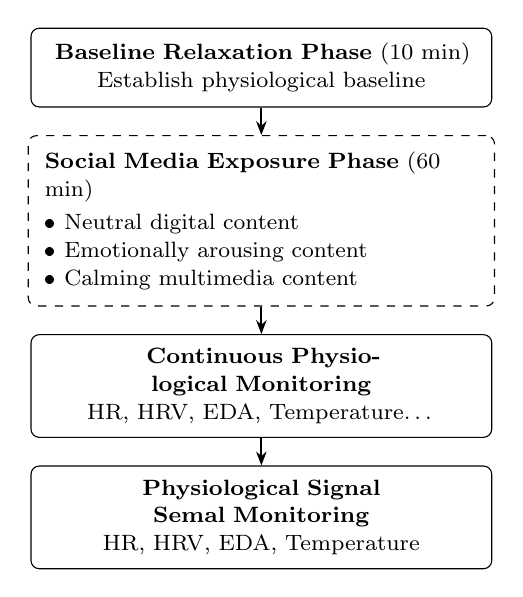
\begin{tikzpicture}[
  font=\fontsize{8}{10}\selectfont,
  box/.style={draw, rounded corners=3pt, text width=5.5cm, align=center, inner sep=5pt, minimum height=1cm},
  dashbox/.style={draw, dashed, rounded corners=3pt, text width=5.5cm, align=left, inner sep=6pt},
  arrow/.style={-{Stealth[length=5pt]}, thick},
  node distance=0.35cm
]
\node[box] (A) {
  \textbf{Baseline Relaxation Phase} (10 min)\\
  Establish physiological baseline
};
\node[dashbox, below=of A] (B) {
  \textbf{Social Media Exposure Phase} (60 min)\\[2pt]
  \textbullet\ Neutral digital content\\
  \textbullet\ Emotionally arousing content\\
  \textbullet\ Calming multimedia content
};
\node[box, below=of B] (C) {
  \textbf{Continuous Physiological Monitoring}\\
  HR, HRV, EDA, Temperature\ldots
};
\node[box, below=of C] (D) {
  \textbf{Physiological Signal Semal Monitoring}\\
  HR, HRV, EDA, Temperature
};
\draw[arrow] (A) -- (B);
\draw[arrow] (B) -- (C);
\draw[arrow] (C) -- (D);
\end{tikzpicture}
\end{center}

\noindent\fontsize{9}{11}\selectfont Fig.\ 2. Experimental protocol for physiological data acquisition during controlled social media exposure.
}
\vspace{4pt}

\begin{enumerate}
  \item Participants were asked to relax themselves for 10-12 mins to establish physiological values.
  \item All the participants were exposed to three categories of social media content:
    \begin{itemize}
      \item Neutral content
      \item Stress inducing content
      \item Relaxing content
    \end{itemize}
  \item Physiological signals were recorded throughout the session.
  \item Motion data was used to filter segments affected by physical activity.
  \item Stress labels were assigned by physiological threshold analysis and baseline derivations.
  \item This protocol ensures consistency among participants.
  \item Raw physiological signals collected often contains noise caused by motion artifacts and environmental sensors. Data is cleaned and several preprocessing steps are applied on the data before generating model.
\end{enumerate}

Steps include:

\begin{enumerate}
  \item To remove high frequency noise low pass and band pass filtering was used.
  \item Average filters were used for Signal smoothing
  \item Accelerometer-based filtering was used for motion artifact reduction
  \item Removal of outliers and corrupted values.
  \item Preprocessing data enhances the signal quality and improves the feature reliability.
\end{enumerate}

\subsection{Feature Extraction}

Meaningful features were extracted from pre-processed data to analyse the stress related patterns.

{\setlength{\parskip}{0pt}
\begin{center}
\fontsize{10}{12}\selectfont
\begin{tabular}{|p{2.0cm}|p{3.8cm}|}
\hline
\textbf{Physiological Signal} & \textbf{Extracted Features} \\
\hline
Heart Rate & Mean, Maximum, Minimum \\
\hline
HRV & SDNN, RMSSD \\
\hline
EDA & Mean conductance, Peak count \\
\hline
Skin Temperature & Mean value, Rate of change \\
\hline
Motion Data & Variance, Signal energy \\
\hline
\end{tabular}
\end{center}
}

\begin{center}
\setlength{\parskip}{0pt}
\textbf{Table III: Extracted Features}
\end{center}

This ensures the use of relative values for physiological signals rather than relying on absolute values.

\subsection{Ensemble-Based Classification}

The overall efficiency of the model, the increase of accuracy, and the robustness are achieved by ensemble learning techniques.

1. \textbf{Base Classifiers:} Three widely used machine learning classifiers are selected as base learners:

\begin{itemize}
  \item Logistic Regression (LR)
  \item Support Vector Machine (SVM)
  \item Random Forest (RF)
\end{itemize}

These classifiers capture both linear and non-linear relationships present in physiological data.

2. \textbf{Voting-Based Ensemble Strategy}

The predicted class probabilities and selection of the class with the highest combined probability served as a method to get the final stress level. The final prediction is obtained by computing the weighted average of individual classifier probabilities and selecting the class with the highest combined probability. This approach improves generalisation and reduces model bias.

3. \textbf{Stacking Based ensemble model}

To enhance the performance of the model, a stacking ensemble model was designed:

\begin{itemize}
  \item Level-0 models: Logistic Regression, SVM, and Random Forest
  \item Level-1 meta-classifier: Logistic Regression
  \item Predictions from the base classifier served as an input for the meta classifier model, allowing the model to learn optimal combinations of individual predictions and to reduce the errors.
\end{itemize}

{\setlength{\parskip}{0pt}
\begin{center}
\fontsize{10}{12}\selectfont
\begin{tabular}{|p{1.6cm}|p{1.4cm}|p{2.5cm}|}
\hline
\textbf{Model} & \textbf{Category} & \textbf{Description} \\
\hline
Logistic Regression & Linear classifier & Baseline stress classification \\
\hline
Support Vector Machine & Kernel-based & Non-linear decision boundaries \\
\hline
Random Forest & Ensemble-based & Feature interaction modeling \\
\hline
Voting Ensemble & Ensemble & Probability-based aggregation \\
\hline
Stacking Ensemble & Meta-learning & Error reduction through model fusion \\
\hline
\end{tabular}
\end{center}
}

\begin{center}
\setlength{\parskip}{0pt}
\textbf{Table IV: Models used}
\end{center}

\vspace{4pt}
\subsection{Evaluation}
\vspace{2pt}

Further, the stress level is divided into three categories:

\begin{enumerate}
  \item High
  \item Moderate
  \item Low
\end{enumerate}

The model assigns stress labels based on learned physiological signals by analysing the patterns corresponding to each class.

The performance of the model was evaluated using standard classification metrics:

\begin{enumerate}
  \item F1 score
  \item Recall
  \item Accuracy
  \item Precision
\end{enumerate}

Then a comparative analysis was done between individual classifiers and ensemble-based models to demonstrate the performance improvement.

This comparison helped in diving in the benefits of ensemble learning approach.

To ensure reproducibility, all experiments were conducted using consistent preprocessing, feature extraction, and evaluation protocols. The ensemble approach enhances reliability by reducing variance and improving robustness across participants.

The stacking ensemble improves performance by combining linear, kernel-based, and tree-based classifiers, allowing complementary decision boundaries to be learned from heterogeneous physiological features. An 80:20 stratified train\textendash test split was used to ensure balanced class representation across stress levels.

Confusion matrix illustrates the classification performance of the stacking ensemble model across three stress levels. The majority of the samples were correctly classified, few discrepancies are present between adjacent stress(low-moderate and moderate-high), which is expected due to physiological similarities in neighboring stress states.

{\setlength{\parskip}{0pt}
\begin{center}
\renewcommand{\arraystretch}{1.5}
\fontsize{9}{11}\selectfont

\hspace{-0.6cm}

\begin{tabular}{|p{1.6cm}|p{0.9cm}|p{0.9cm}|p{0.7cm}|p{0.8cm}|}
\hline
\textbf{Model} & \textbf{Accura- cy (\%)} & \textbf{Preci- sion} & \textbf{Recall} & \textbf{F1-Score} \\
\hline
Logistic Regression & 82.1 & 79.5 & 80.3 & 79.9 \\
\hline
SVM & 84.7 & 81.2 & 83.5 & 82.3 \\
\hline
Random Forest & 87.6 & 85.4 & 86.9 & 86.1 \\
\hline
Voting Ensemble & 87.3 & 87.0 & 86.2 & 86.4 \\
\hline
Stacking Ensemble & 89.6 & 89.1 & 88.0 & 88.1 \\
\hline
\end{tabular}

\end{center}
}

\begin{center}
\setlength{\parskip}{0pt}
\textbf{Table V: Performance of the models}
\end{center}

{\setlength{\parskip}{0pt}
\begin{center}
\fontsize{10}{12}\selectfont
\begin{tabular}{|p{1.7cm}|p{1.1cm}|p{1.3cm}|p{1.0cm}|}
\hline
\textbf{Actual/ Predicted} & \textbf{Low Stress} & \textbf{Moderate Stress} & \textbf{High Stress} \\
\hline
\textbf{Low Stress}      & 145 & 8   & 2   \\
\hline
\textbf{Moderate Stress} & 9   & 132 & 9   \\
\hline
\textbf{High Stress}     & 3   & 7   & 135 \\
\hline
\end{tabular}
\end{center}
}

\begin{center}
\setlength{\parskip}{0pt}
\textbf{Table VI: Confusion Matrix}
\end{center}

% ── V. CONCLUSION ────────────────────────────────────────────
\section{Conclusion}

This work introduces a practical method to identify stress caused by social media usage by combining data from wearable sensors with machine learning techniques. Instead of relying on opinions or questionnaires, the system observes real body signals such as heart rate, skin response, and temperature, which reflect stress more naturally and honestly.

The study shows that different kinds of online content affect the human body in different ways. Stress-related content leads to noticeable physical changes, while calming content helps the body return to a relaxed state. Careful data cleaning and feature selection helped capture these changes accurately. Using multiple models together improved the reliability and stability of stress prediction for different individuals.

In summary, analyzing how the body reacts while consuming digital content offers a simple, non-intrusive, and effective way to detect stress. This approach shows potential as a supportive stress awareness and monitoring framework. With further improvements and real-time deployment, it can help users become more aware of their stress levels and take timely action to manage them better.

% ── VI. LIMITATIONS AND FUTURE WORK ─────────────────────────
\section{Limitations and Future Work}

Despite the promising results, this study has several limitations that need to be acknowledged. First, the dataset was collected among a small group of participants(200) and within narrow age range(18-25 years). This limits the generalizability of the proposed model to broader populations.

Second, the experiment was conducted in an isolated lab where participants were exposed to predefined categories of social media content. Real-world social media usage is more complex, dynamic and influenced by multiple factors that are not mentioned in this study.

Third, stress labelling was done using threshold analysis rather than clinical diagnosis. Therefore, the predicted stress levels should be interpreted as risk indicators rather than clinical assessments.

Additionally, the use of ensemble and stacking-based models on a limited dataset may introduce the problem of overfitting, despite the use of consistent preprocessing and evaluation protocols.

Future work involves expanding the dataset to diverse demographic groups, integrating real-time social media usage metrics, screen time and application-level activity, and explainable machine learning techniques to enhance the model transparency and performance. Furthermore, the ethical approval and long-term real-time deployment studies will be explored to evaluate system effectiveness in real-life scenarios.

\bibliographystyle{IEEEtran}
\bibliography{references}

\end{multicols}
\end{document}
